
CCSTM's implementation as an unprivileged library introduces several
overheads when compared to a bytecode rewriting STM or modified VM:
\type{Ref} adds a level of indirection; JVM erasure adds boxing overheads
for \xtype{Ref}{T} when \typeparam{T} is a primitive type; avoiding boxing
for long-term storage requires that the underlying memory locations
be accessed through virtual methods; dynamic scoping involves a hash
table lookup, either implicitly inside \type{ThreadLocal} or explicitly
with a \type{Thread} key; and low-level atomic operations performed by
the STM cannot use the unchecked primitives in \code{sun.misc.Unsafe}.
The actual impact of these overheads, however, is reduced or eliminated
by the compiler optimizations of a modern JVM and the out-of-order
superscalar pipeline of a modern processor.

To verify that CCSTM's library-based design does not impose a prohibitive
performance penalty, we compared it to Deuce STM and Multiverse, STMs for
the JVM that perform bytecode rewriting during class
loading~\cite{deucestm,multiverse}.
We performed a direct encoding of Deuce STM's bank benchmark into
Scala+CCSTM, and compared this version to the Java original running
under the bytecode rewriting STMs.  (While the example code in this paper uses an
immutable \type{Money} numeric type, the evaluated benchmark uses 32-bit
floating point values like the original.)  Deuce STM provides two algorithms,
TL2 and LSA, each of which has optional contention management (CM).
For each configuration and thread count, we report the throughput of a Deuce STM algorithm
as the maximum of the throughput with no CM or with CM (Polka for TL2, Timestamp for
LSA).
For almost all configurations we tested, CM reduced
throughput.  CCSTM and Multiverse were tested using their default
configuration.
The bank benchmark includes its own harness, which we configured so
that no overdrafts were triggered.  We used a 20 second warmup, and
then measured the number of transactions committed during 10 seconds,
averaging across three invocations of the JVM.

Experiments were run on a Dell Precision T7500n with two quad-core
2.66Ghz Intel Xeon X5550 processors, and 24GB of RAM.  Hyper-Threading was
enabled, yielding a total of 16 hardware thread contexts.  We used Scala
version 2.8.0.Beta1.  We ran our experiments in
Sun's Java~SE Runtime Environment, build 1.6.0\_16-b01, using the HotSpot
64-Bit Server VM with dynamic escape analysis and compressed object pointers
enabled.  Deuce STM was version 1.3.0.  Multiverse was version 0.4.

For the low-contention
experiment (Figure~\ref{fig:lowcont}) we set the number of accounts
to 64 times the number of threads.  For the high-contention experiment
(Figure~\ref{fig:highcont}) we set the number of accounts to the number of
threads.  Single-threaded execution is not included in the high-contention
setup, as it has no contention.  Because at most 16 threads are executing
at any time, high-contention runs have fewer conflicts at 32 and 64
threads than for lower thread counts, and so can continue to scale so long as
blocked threads do not consume too many resources.  This effect is present
to a lesser degree for the low-contention runs, where CCSTM's throughput
continues to rise gradually as its rollback rate
drops from 1.0\% at 16 threads to 0.5\% at 32 and 0.3\% at 64.

\begin{figure}
  \centering 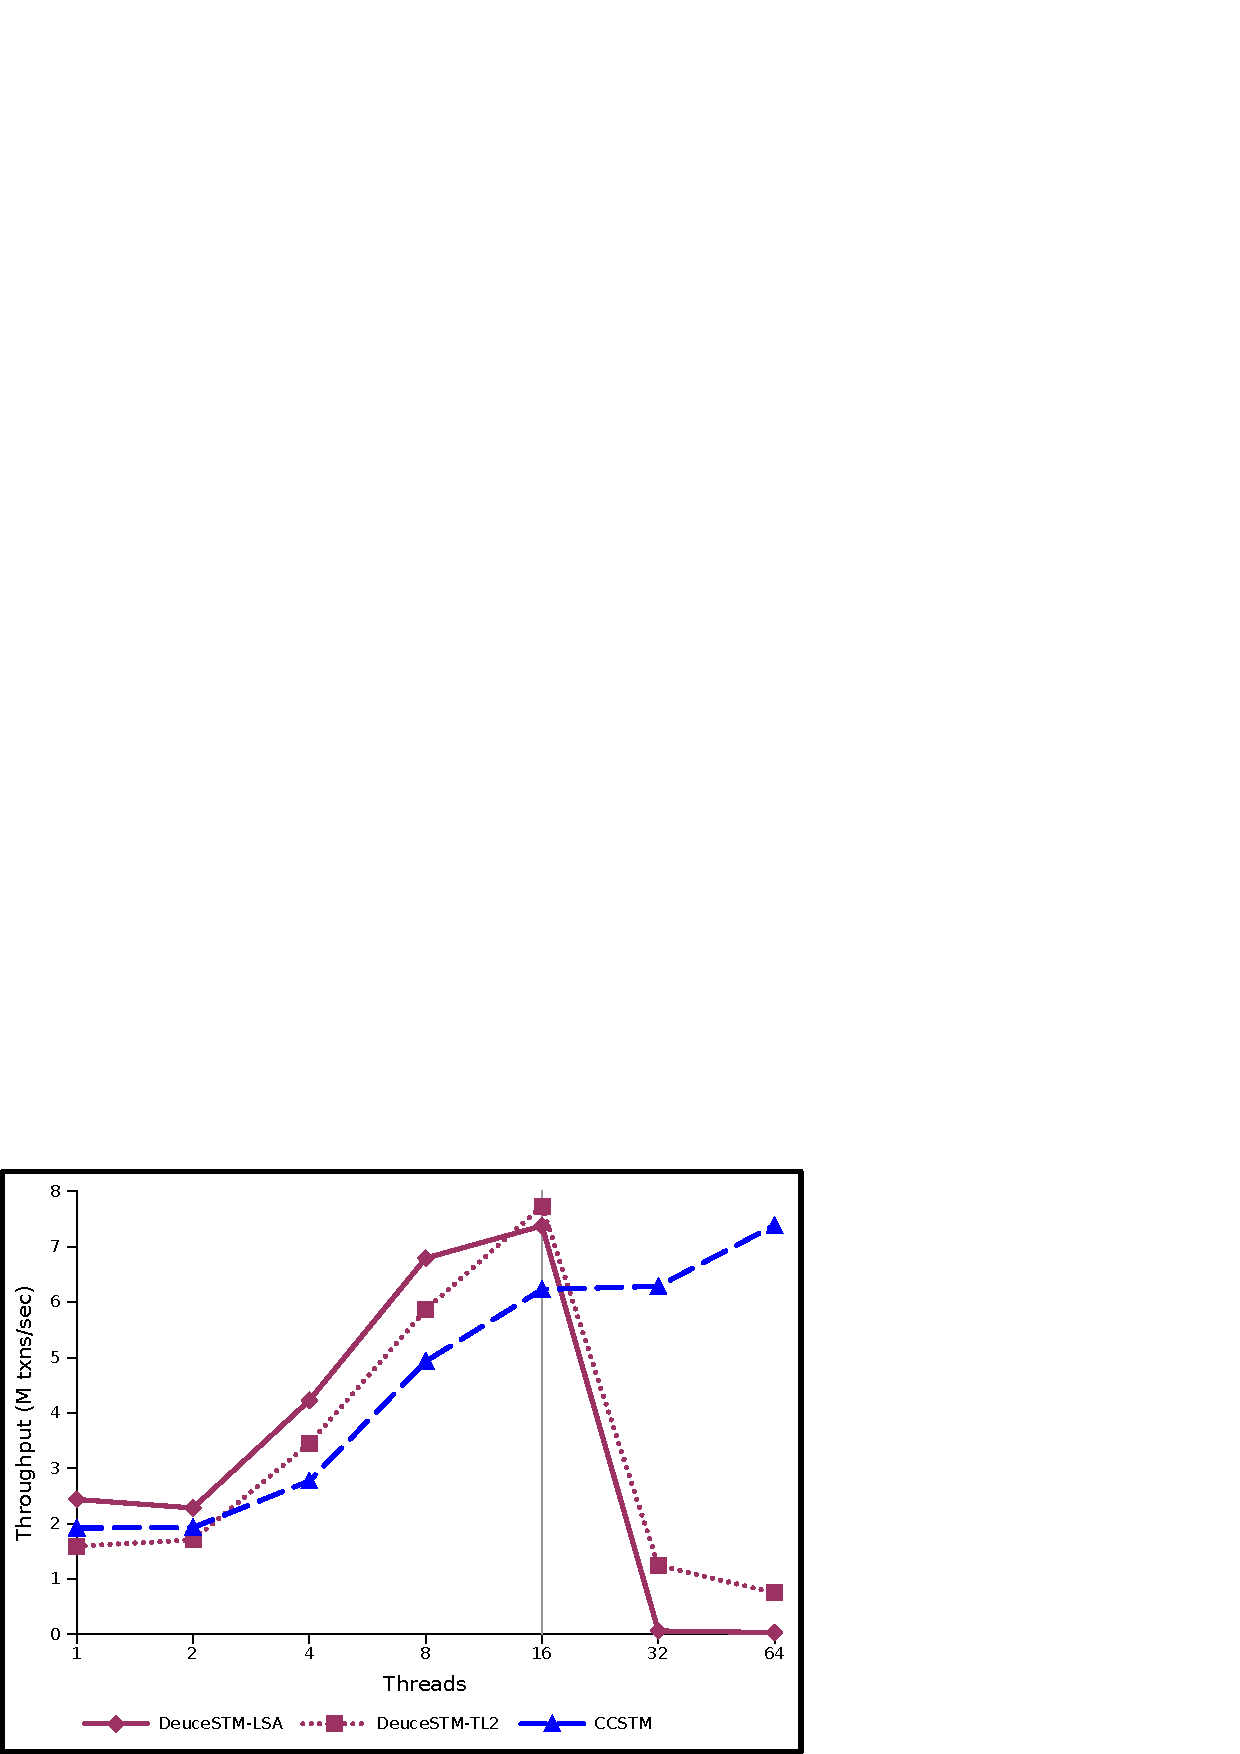
\includegraphics[clip=true,width=3in]{build/low_cont}

\caption{Throughput for the bank benchmark in a low contention scenario,
on a machine with 16 hardware thread contexts.  The number of accounts
is 64 times the number of threads.}

  \label{fig:lowcont}
\end{figure}

\begin{figure}
  \centering 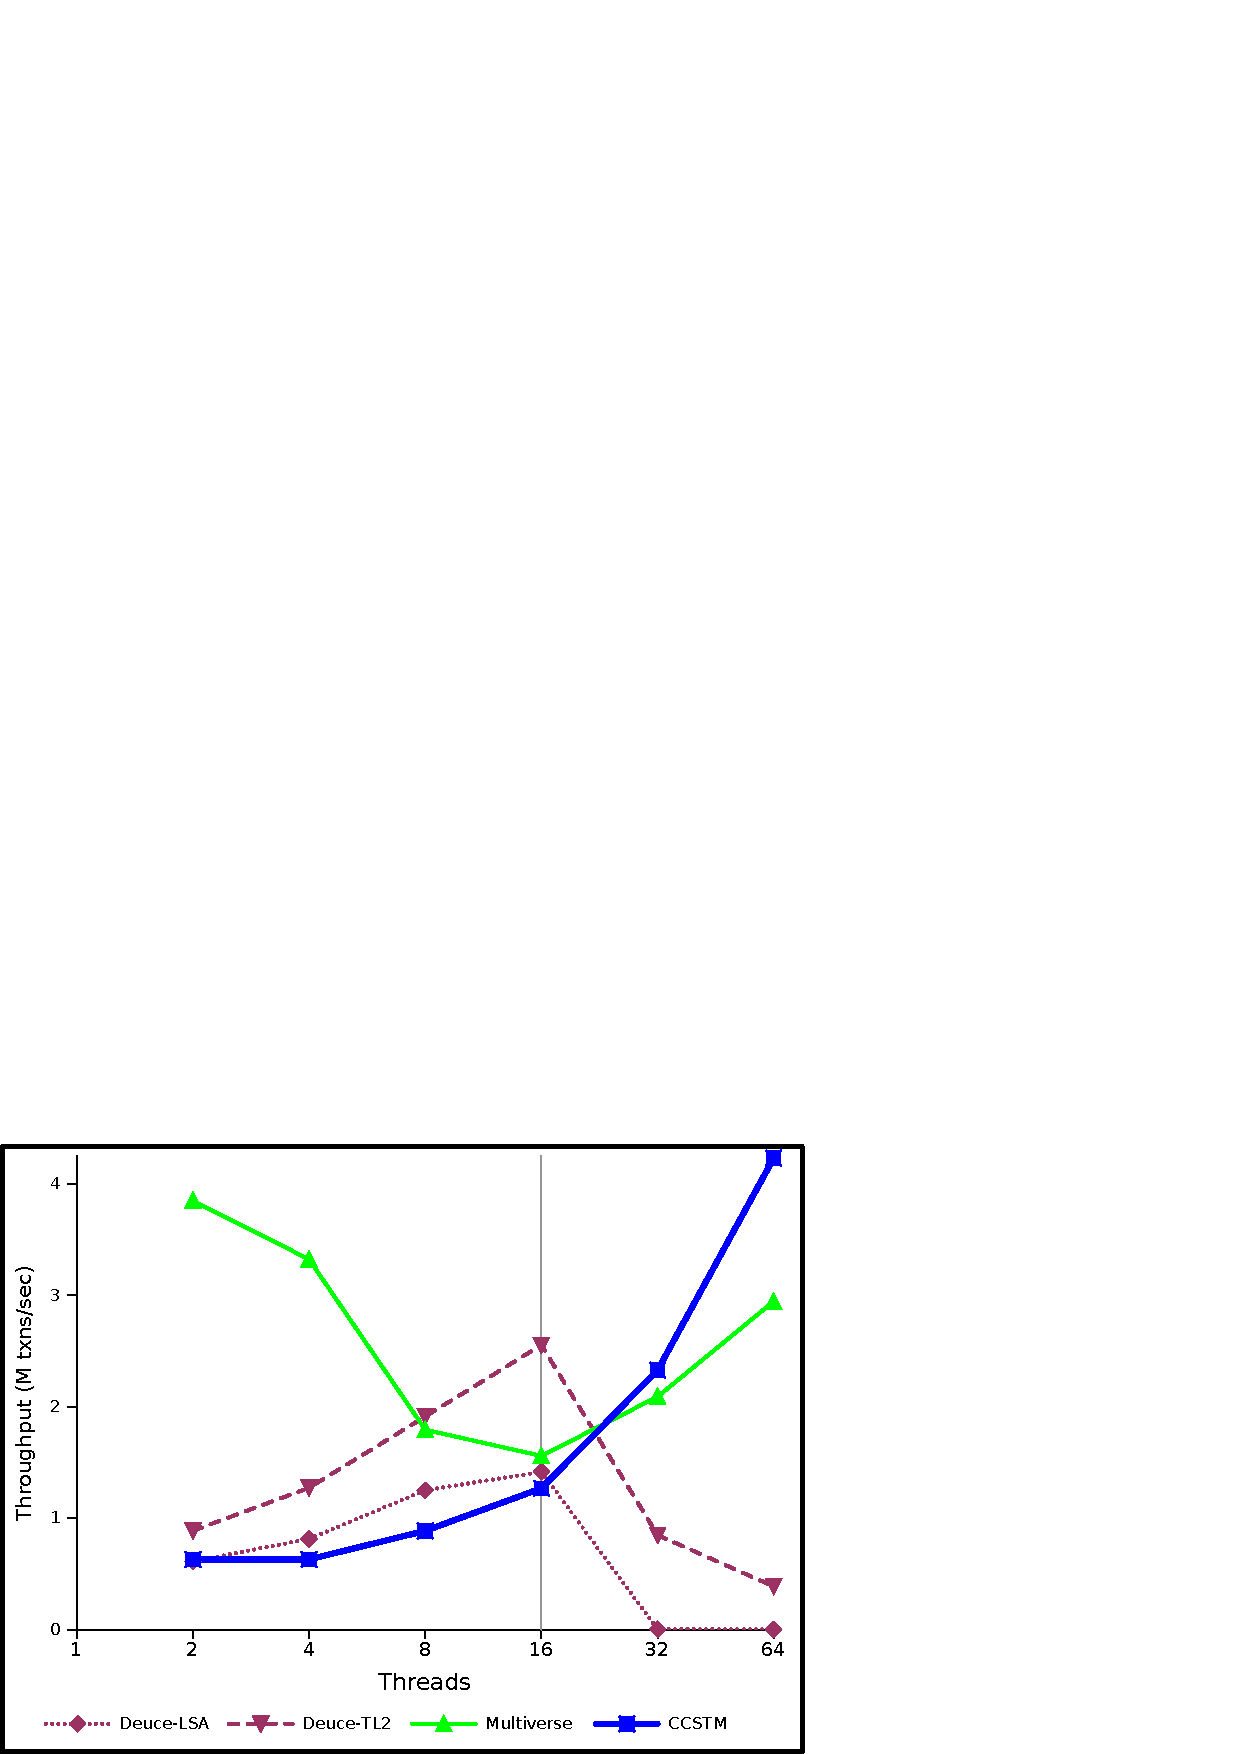
\includegraphics[clip=true,width=3in]{build/high_cont}

\caption{Throughput for a high contention scenario.  The number of accounts is
equal to the number of threads.  Each transaction touches two accounts.}

  \label{fig:highcont}
\end{figure}

For low contention configurations, Deuce STM and CCSTM have similar
performance and scalability, so long as the multithreading level is less
than or equal to one.  Under high contention Deuce STM substantially
outperforms CCSTM, so long as each thread gets its own hardware context.
This is because Deuce STM uses busy-waiting, which avoids context switches
for blocked threads.  At thread counts 32 and 64, however, threads must
share processing resources and this strategy results in a catastrophic
performance drop off.  Multiverse uses an exponential back off algorithm
using \code{Thread.sleep}.  This approach handles high multithreading
levels better than busy-waiting, but results in extra context switches as
threads awake to recheck their blocking condition.  Sleeping works very well
for low thread counts
of the high-contention configuration, because
it leads to intervals of uncontended single-threaded execution.
CCSTM's blocking synchronization implementation is the most
expensive at low thread counts, but it yields a robust scaling curve.

The three STMs have different algorithms, feature sets and engineering
tradeoffs, so these experiments do not allow us to exactly measure
the overhead imposed by the library-only design.  They do demonstrate,
however, that the practical overheads that exist are small enough to be
tolerable.  We leave as future work a breakdown of the costs inside CCSTM.

